
\documentclass[12pt]{article}
\usepackage{graphicx}
\title{Ch 121a Proposal}
\author{Patryk Kozlowski}
\date{\today}
\begin{document}
\section{Perovskites}
\subsubsection{Structure}
The perovskite stucture is ABO3, where A is a large cation, B is a smaller cation, and O is an oxygen anion. The B cation is typically a transition metal, and the A cation is typically an alkali metal or alkaline earth metal. The structure is face-centered cubic, with the B cation at the center of the cube, the A cation at the corners of the cube, and the O anion at the center of each face of the cube. The structure is shown in Figure 1.
\begin{figure}
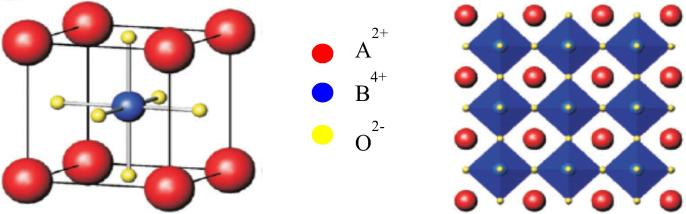
\includegraphics[width=\linewidth]{perovskite.png}
\caption{The ideal face-centered cubic perovskite structure. \cite{assirey2019perovskite}}
\label{fig:perovskite}
\end{figure}
\subsubsection{Applications}
Perovskites have shown potential as efficient heterogeneous catalysts, and could be used to replace platinum-group metal (PGM) catalysts as they are cheaper and easier to synthesize. Additionally, the structure of perovskites allows for a wide range of substituting and doping, allowing to tailor their properties to better target applications \cite{royer2014perovskites}.
\section{Objectives}
I will be using VASP to compute surface energies of perovskites, first using DFT and then using the wavefuntion-based methods HF and MP2. I will compare my results to experimental data from the literature.
\section{Method}
\subsection{Find experimental data for comparison}
Materials Project looks promising.
\subsubsection{Choice of perovskite/quantity}
Leaning toward computation of surface energies, as opposed to adsorption energies. Thinking that it will be good to focus on the material itself, and leave the adsorbates out.  the materials I have in mind are LaMnO3, LaFeO3, and SrTiO3. Thinking to choose one of these three, and then choose a quantity to compute for that material. How many systems do I want to choose for study given my somewhat limited time frame (this isn't a SURF project that I can spend 45 hrs/week for 10 weeks on)?
\subsection{Perform DFT calculations}
\subsubsection{Choice of DFT functional}
any advice here? I could try and educate myself on this point, but thinking that you gus might have easy answer that might be most appropriate.
\subsection{Basis choice}
To be compatible with both DFT and later the wavefunction-based methods HF and MP2. Any advice here?
\subsubsection{Choice of k-point mesh}
Any advice here? Or do I simply need to look through the computational literature to find out what has been done in the past? The later is probably good idea for me to look into, but I am not completely aware of the timeline for Ch121 project as a whole, as you probably are.
\subsection{Perform HF and MP2 calculations}
I was speaking with Charles and we agreed that this might be a good continuation into Ch121b, where I will start on DFT now in Ch121a, and then move on to HF and MP2 in Ch121b.
\bibliographystyle{unsrt}
\bibliography{citations}
\end{document}
